%%%%%%%%%%%%%%%%%%%%%%%%%%%%%%%%%%%%

\section{連続分布}

%%%%%%%%%%%%%%%%%%%%%%%%%%%%%%%%%%%%

\begin{frame}[shrink=15]
\frametitle{連続分布}

\begin{itemize}

\item 以下は米国成人の身長の分布のヒストグラムである。

\item 陰影のついたビンに含まれるデータの割合が、無作為に選ばれた米国成人の身長が180cmから185cm（約5'11''から6'1''）である確率を示す。

\end{itemize}

\begin{center}
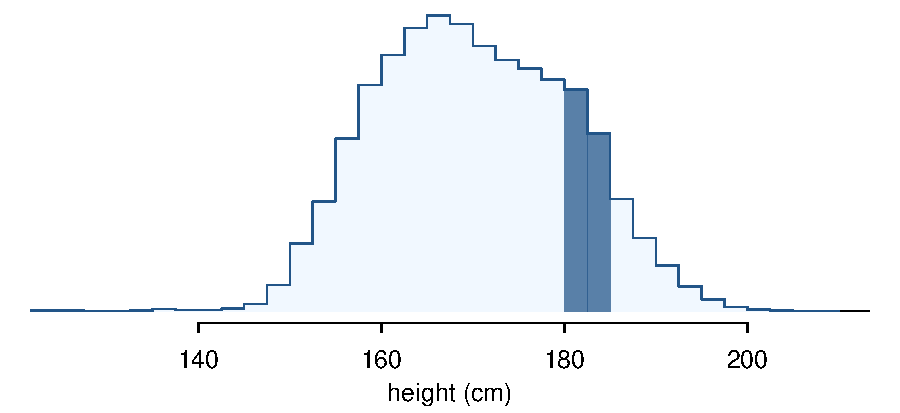
\includegraphics[width=\textwidth]{3-5_continuous_distributions/figures/usHeightsHist180185/usHeightsHist180185}
\end{center}


\end{frame}

%%%%%%%%%%%%%%%%%%%%%%%%%%%%%%%%%%%%

\subsection{ヒストグラムから連続分布へ}

\begin{frame}
\frametitle{ヒストグラムから連続分布へ}

身長は連続数値変数であるため、その\hl{確率密度関数}は滑らかな曲線となる。

\begin{center}
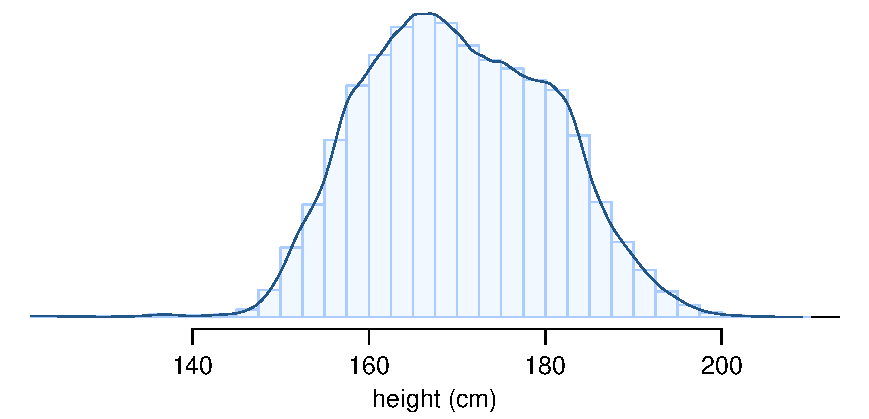
\includegraphics[width=\textwidth]{3-5_continuous_distributions/figures/fdicHeightContDist/fdicHeightContDist}
\end{center}

\end{frame}

%%%%%%%%%%%%%%%%%%%%%%%%%%%%%%%%%%%%

\subsection{連続分布からの確率}

\begin{frame}[shrink=10]
\frametitle{連続分布からの確率}

したがって、無作為に選ばれた米国成人の身長が180cmから185cmである確率は、曲線の下の陰影部分の面積としても推定できる。

\begin{center}
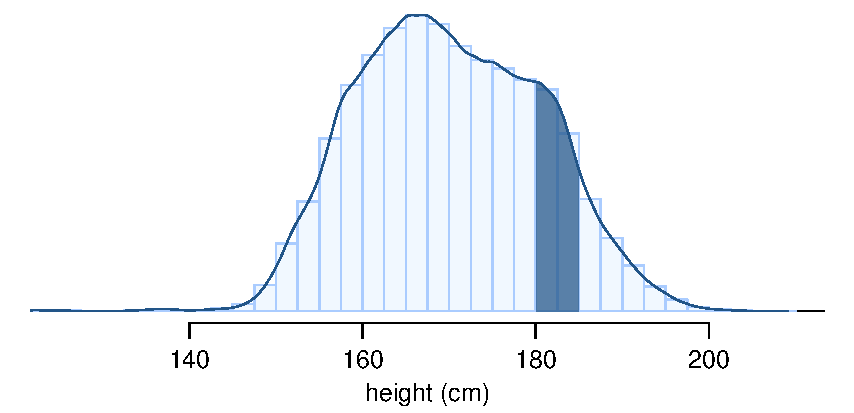
\includegraphics[width=\textwidth]{3-5_continuous_distributions/figures/fdicHeightContDistFilled/fdicHeightContDistFilled}
\end{center}


\end{frame}

%%%%%%%%%%%%%%%%%%%%%%%%%%%%%%%%%%%%

\begin{frame}
\frametitle{定義によれば…}

連続確率は「曲線の下の面積」として推定されるため、ある人の身長がちょうど180cm（または任意の特定の値）である確率は0と定義される。

\begin{center}
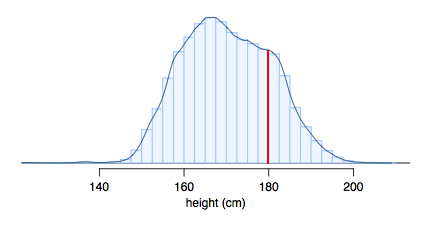
\includegraphics[width=0.8\textwidth]{3-5_continuous_distributions/figures/fdicHeightContDist180}
\end{center}

\end{frame}

%%%%%%%%%%%%%%%%%%%%%%%%%%%%%%%%%%%%
